\section{Evaluation}
\label{sec:eval}

\subsection{Setup}
We evaluate on Qwen2.5-1.5B-Instruct (MLX int4) on an Apple~M3 with $8.59$\,GB unified memory
(full details in Appendix~\ref{app:repro}). The probe is needle-in-a-haystack
(NIAH)~\cite{kamradt2023niah}: a planted passcode (\texttt{OMEGA-7741-DELTA}) is buried in a
filler document and the same prompt, built once per context length from the Qwen2.5 tokenizer, is
fed verbatim to every configuration at $4$k, $8$k, $16$k, $32$k, and $64$k tokens. Decode is
fixed-length greedy ($128$ tokens, EOS ignored) so throughput is directly comparable. We compare
three configurations on identical prompts:
\begin{itemize}[leftmargin=1.4em,itemsep=1pt]
  \item \textbf{\diffkv{} compressed} --- the runtime's real sparse decode
  (\texttt{DIFFKV\_COMPRESSED\_DECODE=1}); the primary result.
  \item \textbf{Exact ablation} --- the same \diffkv{} prefill and store, but decode computed over
  the retained native cache (\texttt{=0}); an upper bound on what perfect-fidelity retrieval from
  this store would achieve.
  \item \textbf{Dense} --- stock \texttt{mlx\_lm} with a full KV cache (same int4 weights, same
  engine); the no-compression control.
\end{itemize}
Memory is reported as the MLX allocator peak (global, prefill-dominated) and a decode-phase peak
(counter reset at the prefill$\to$decode boundary), plus the analytic KV-state footprint of the
store versus a dense full cache. We answer five questions.

\subsection{E1 --- KV-state footprint (the memory result)}
Figure~\ref{fig:g1} and Table~\ref{tab:main} show the headline. \diffkv{}'s occupied KV state grows
from $0.028$\,GB at $4$k to $0.20$\,GB at $64$k, while the dense full cache for the same sequences
grows from $0.117$\,GB to $1.88$\,GB---a gap that widens from $4.1\times$ to $9.3\times$ as context
grows, approaching the per-block $10.25\times$ bound (Table~\ref{tab:budget}) as a larger fraction
of the sequence leaves the recency window. The compressed pool is moreover \emph{pre-allocated and
bounded}: its capacity is fixed at $\approx\!0.2$\,GB irrespective of context, so the store cannot
grow past it. This is the property the rest of the system exploits.

\begin{figure}[t]
  \centering
  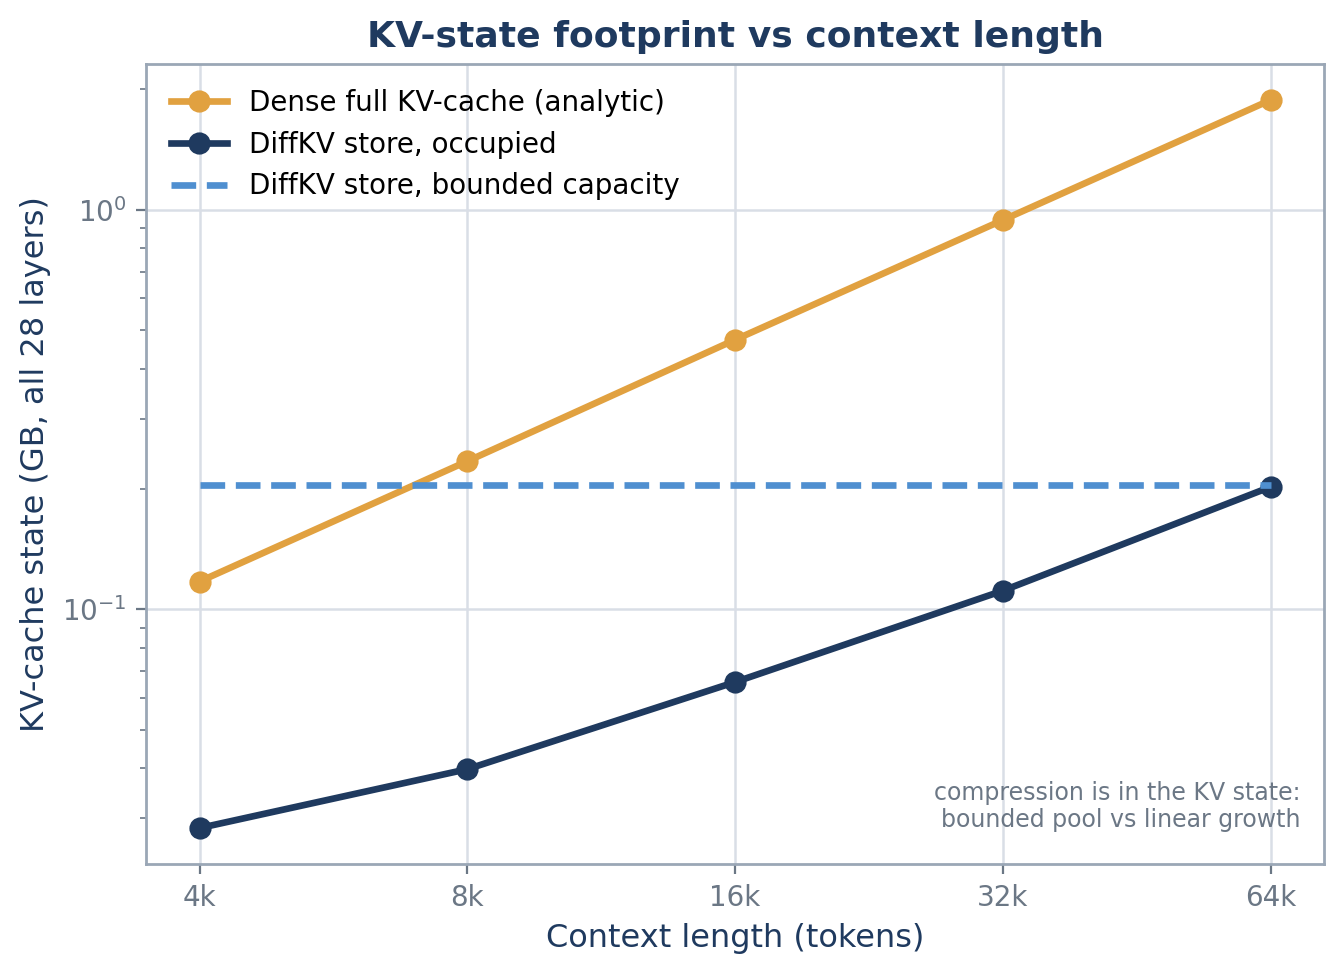
\includegraphics[width=0.92\linewidth]{figures/g1_kv_footprint.png}
  \caption{KV-state footprint vs.\ context (all $28$ layers). \diffkv{}'s store is bounded and far
  below the linearly growing dense cache; the gap widens toward the per-block $10\times$ bound as
  more tokens are compressed. Analytic bytes from the live store; no estimation.}
  \label{fig:g1}
\end{figure}

\begin{table}[t]
\centering
\caption{Main results: \diffkv{} compressed decode (primary), exact decode (upper-bound ablation),
and the dense baseline. All measured on the same Apple~M3; greedy $128$-token decode. The dense
baseline was measured to $32$k; its $64$k full cache ($1.88$\,GB) plus weights and prefill
activations exceeds the safe budget on this device.}
\label{tab:main}
\small
\begin{tabular}{lrrrrr}
\toprule
Metric & 4k & 8k & 16k & 32k & 64k \\
\midrule
\multicolumn{6}{l}{\textit{DiffKV compressed sparse decode (primary)}}\\
\quad Prefill (s) & 9.4 & 20.7 & 47.1 & 118.9 & 432.5 \\
\quad Decode (tok/s) & 16.9 & 10.8 & 9.3 & 6.8 & 3.9 \\
\quad Decode-phase MLX peak (GB) & 1.82 & 1.79 & 2.03 & 2.50 & 3.44 \\
\quad KV store, occupied (GB) & 0.054 & 0.096 & 0.181 & 0.346 & 0.676 \\
\quad Needle recovered & \cmark & \cmark & \cmark & \cmark & \cmark \\
\midrule
\multicolumn{6}{l}{\textit{Exact full-KV decode (upper-bound ablation)}}\\
\quad Decode (tok/s) & 38.0 & 35.1 & 31.5 & 21.6 & 8.6 \\
\quad Needle recovered & \cmark & \cmark & \cmark & \cmark & \cmark \\
\midrule
\multicolumn{6}{l}{\textit{Dense baseline (mlx\_lm, full KV)}}\\
\quad Prefill (s) & 5.1 & 11.1 & 27.4 & 92.3 & -- \\
\quad Decode (tok/s) & 66.9 & 61.7 & 47.3 & 30.1 & -- \\
\quad Full KV-cache (GB, analytic) & 0.117 & 0.235 & 0.473 & 0.942 & 1.881 \\
\quad Needle recovered & \cmark & \cmark & \cmark & \cmark & -- \\
\bottomrule
\end{tabular}
\end{table}

\subsection{E2 --- Context reach}
\diffkv{} compressed processes the full $64$k prompt ($65{,}615$ tokens) within budget: its store
caps at $\approx\!0.2$\,GB and the decode-phase peak is $2.97$\,GB
(Table~\ref{tab:detail}), well under the device limit. The bounded pool ($M\bs=65{,}536$ compressed
tokens plus a $768$ window) is sized precisely to reach this context. The dense baseline, whose
cache alone is $1.88$\,GB at $64$k on top of weights and the prefill peak, is the configuration that
runs out of headroom first---the qualitative capability gap that motivates the design.

\subsection{E3 --- Prefill time}
Prefill is exact in all configurations and scales near-linearly with context
(Fig.~\ref{fig:g4}); \diffkv{} adds the streaming SVD on top of the same attention, so its prefill
is the slowest of the MLX configurations ($8.1$\,s at $4$k to $313$\,s at $64$k). Prefill is the
dominant wall-time cost at large context and the main target for future work
(\S\ref{sec:limitations}).

\subsection{E4 --- Decode throughput}
Figure~\ref{fig:g3} and Table~\ref{tab:main} show the throughput trade-off. \diffkv{} compressed
decode is roughly flat at $\approx\!8$\,tok/s ($8.0/8.1/8.2/8.0/6.8$ across $4$k--$64$k), consistent
with per-token cost that is linear in the number of blocks with a small rank-weighted constant
(\S\ref{sec:decode}). The exact ablation on the same store decodes far faster
($42.8/40.3/35.2/24.2/17.6$\,tok/s across $4$k--$64$k) and the dense baseline faster still
($66.9/61.7/47.3/30.1$\,tok/s, $4$k--$32$k). Because the ablation differs from compressed \emph{only} in the decode
kernel, the gap is attributable to the compressed-kernel dispatch, not to the compression---a
hand-written fused kernel is the path to closing it (\S\ref{sec:limitations}).

\begin{figure}[t]
  \centering
  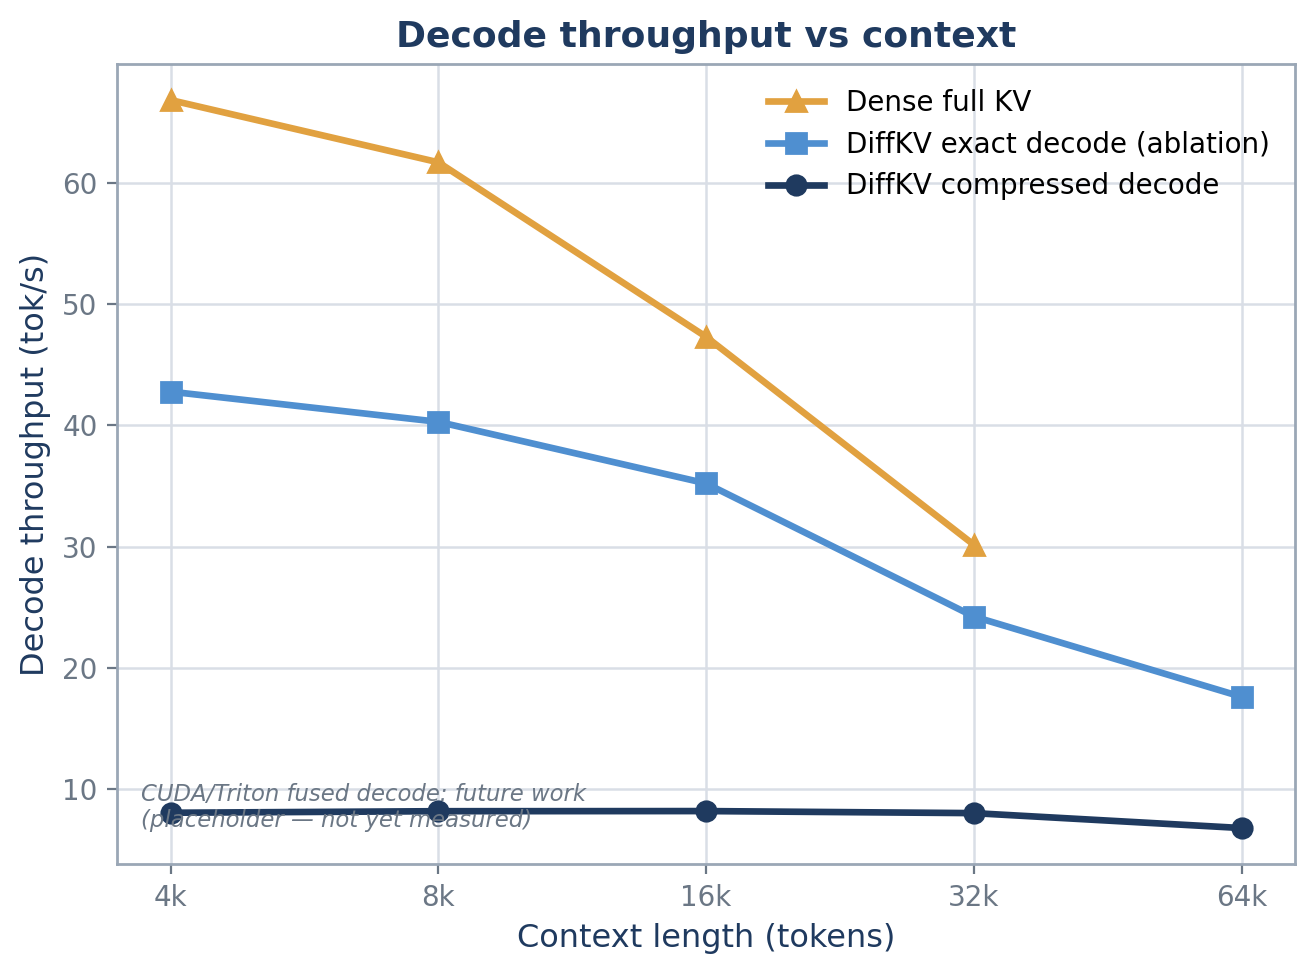
\includegraphics[width=0.92\linewidth]{figures/g3_decode_tps.png}
  \caption{Decode throughput vs.\ context. Compressed decode is flat and slow; the exact ablation
  recovers dense-like throughput, localizing the gap to the kernel. A CUDA/Triton fused-decode
  series can be added here without restructuring (future work).}
  \label{fig:g3}
\end{figure}

\begin{figure}[t]
  \centering
  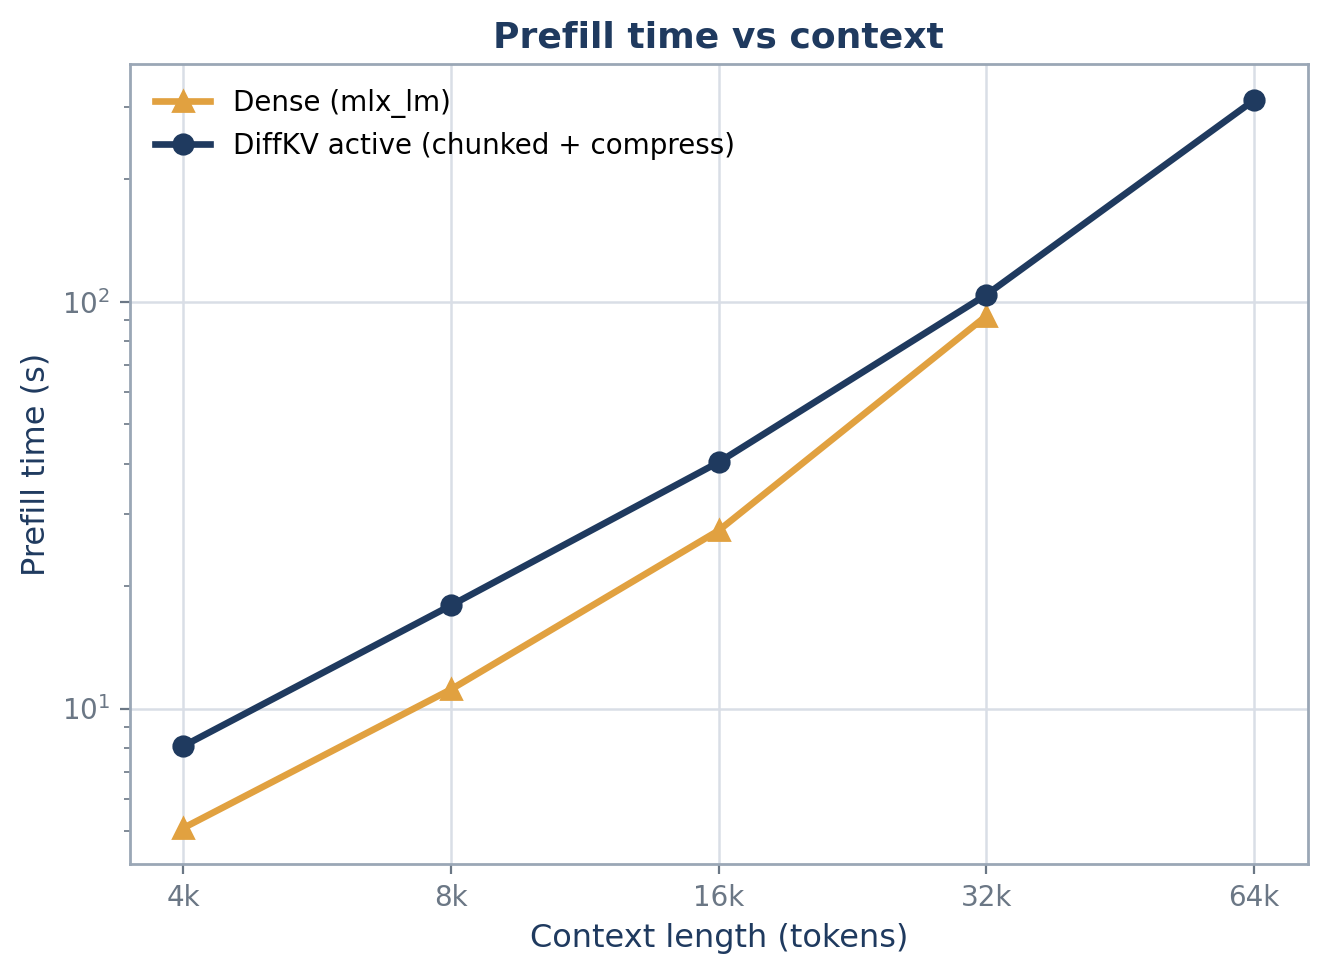
\includegraphics[width=0.92\linewidth]{figures/g4_prefill.png}
  \caption{Prefill time vs.\ context (log scale). Exact attention plus streaming SVD; near-linear
  growth, slowest among the MLX configurations.}
  \label{fig:g4}
\end{figure}

\subsection{E5 --- Needle correctness}
This is where the compressed path's current limitation is sharpest. \diffkv{} compressed
\emph{fails} to reproduce the buried passcode at every context ($4$k--$64$k), while the exact
ablation on the identical store recovers it at every measured context (Table~\ref{tab:main}). The
ablation isolates the cause to rank-$16$ truncation of needle-bearing blocks rather than to the
runtime: once the needle's block is compressed, the low-rank reconstruction does not retain enough
of the single-token detail for greedy decoding to emit the exact string, and the unseeded
randomized SVD makes the (wrong) output non-deterministic. We report this as the central open
problem (\S\ref{sec:fidelity}, \S\ref{sec:limitations}), not as a footnote.

\subsection{Allocator peak and the combined view}
Figure~\ref{fig:g2} reports the MLX allocator peak, which is nearly identical across all three
configurations at matched context because it is set during prefill; compression lowers the
\emph{decode-phase} resident memory, not this peak (\S\ref{sec:analysis}). Figure~\ref{fig:g5}
combines footprint, throughput, and prefill in one view.

\begin{figure}[t]
  \centering
  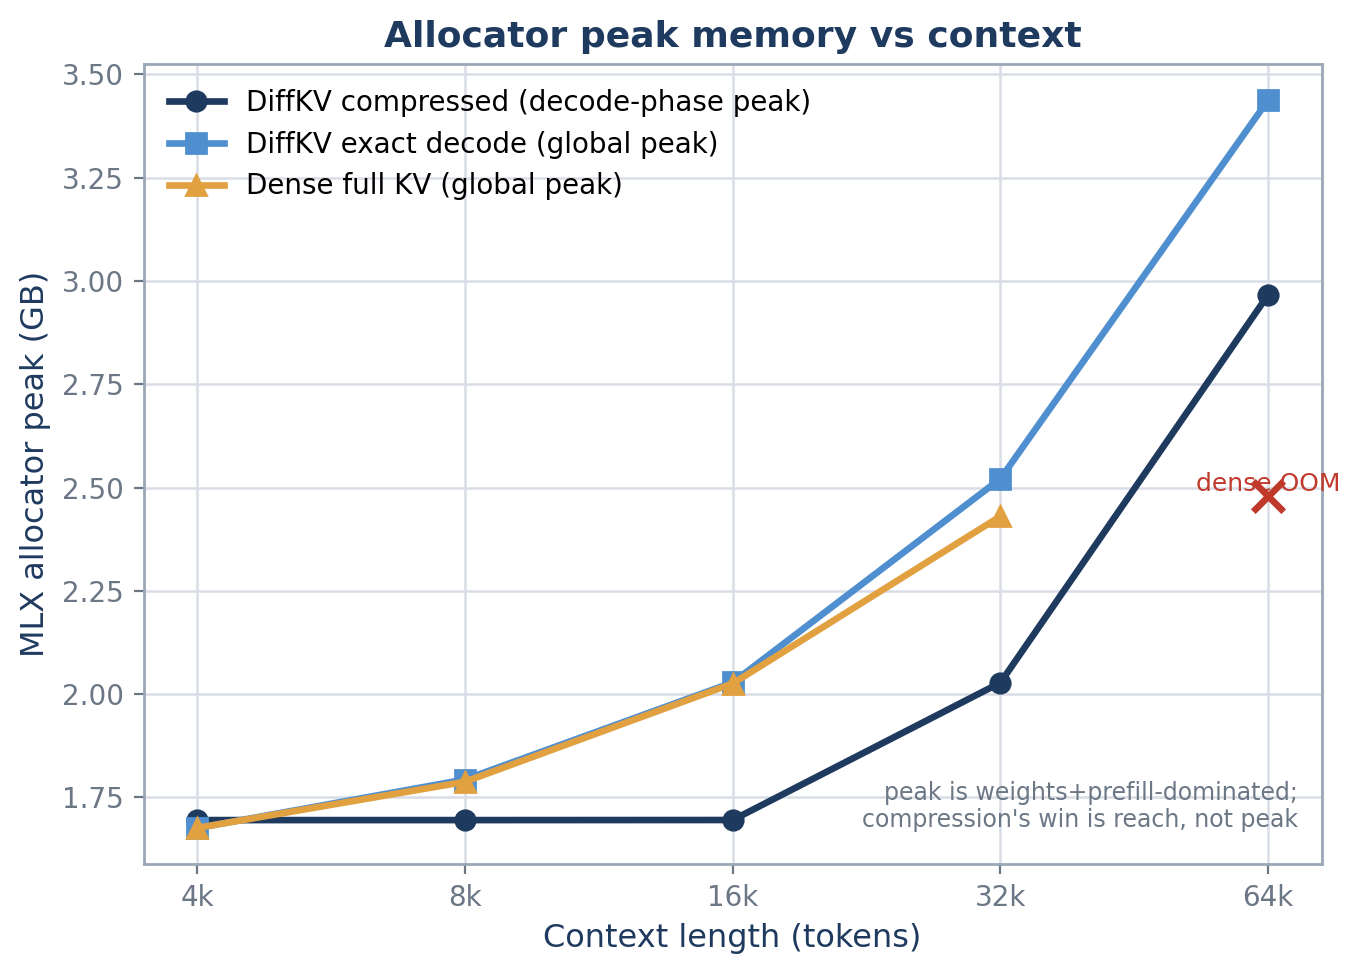
\includegraphics[width=0.92\linewidth]{figures/g2_mx_peak.png}
  \caption{MLX allocator peak vs.\ context. Nearly identical across configurations---peak is
  weights- and prefill-dominated. Compression's win is context reach and steady-state decode
  memory, not the global peak; we report it honestly rather than overstate a peak reduction.}
  \label{fig:g2}
\end{figure}

\begin{figure*}[t]
  \centering
  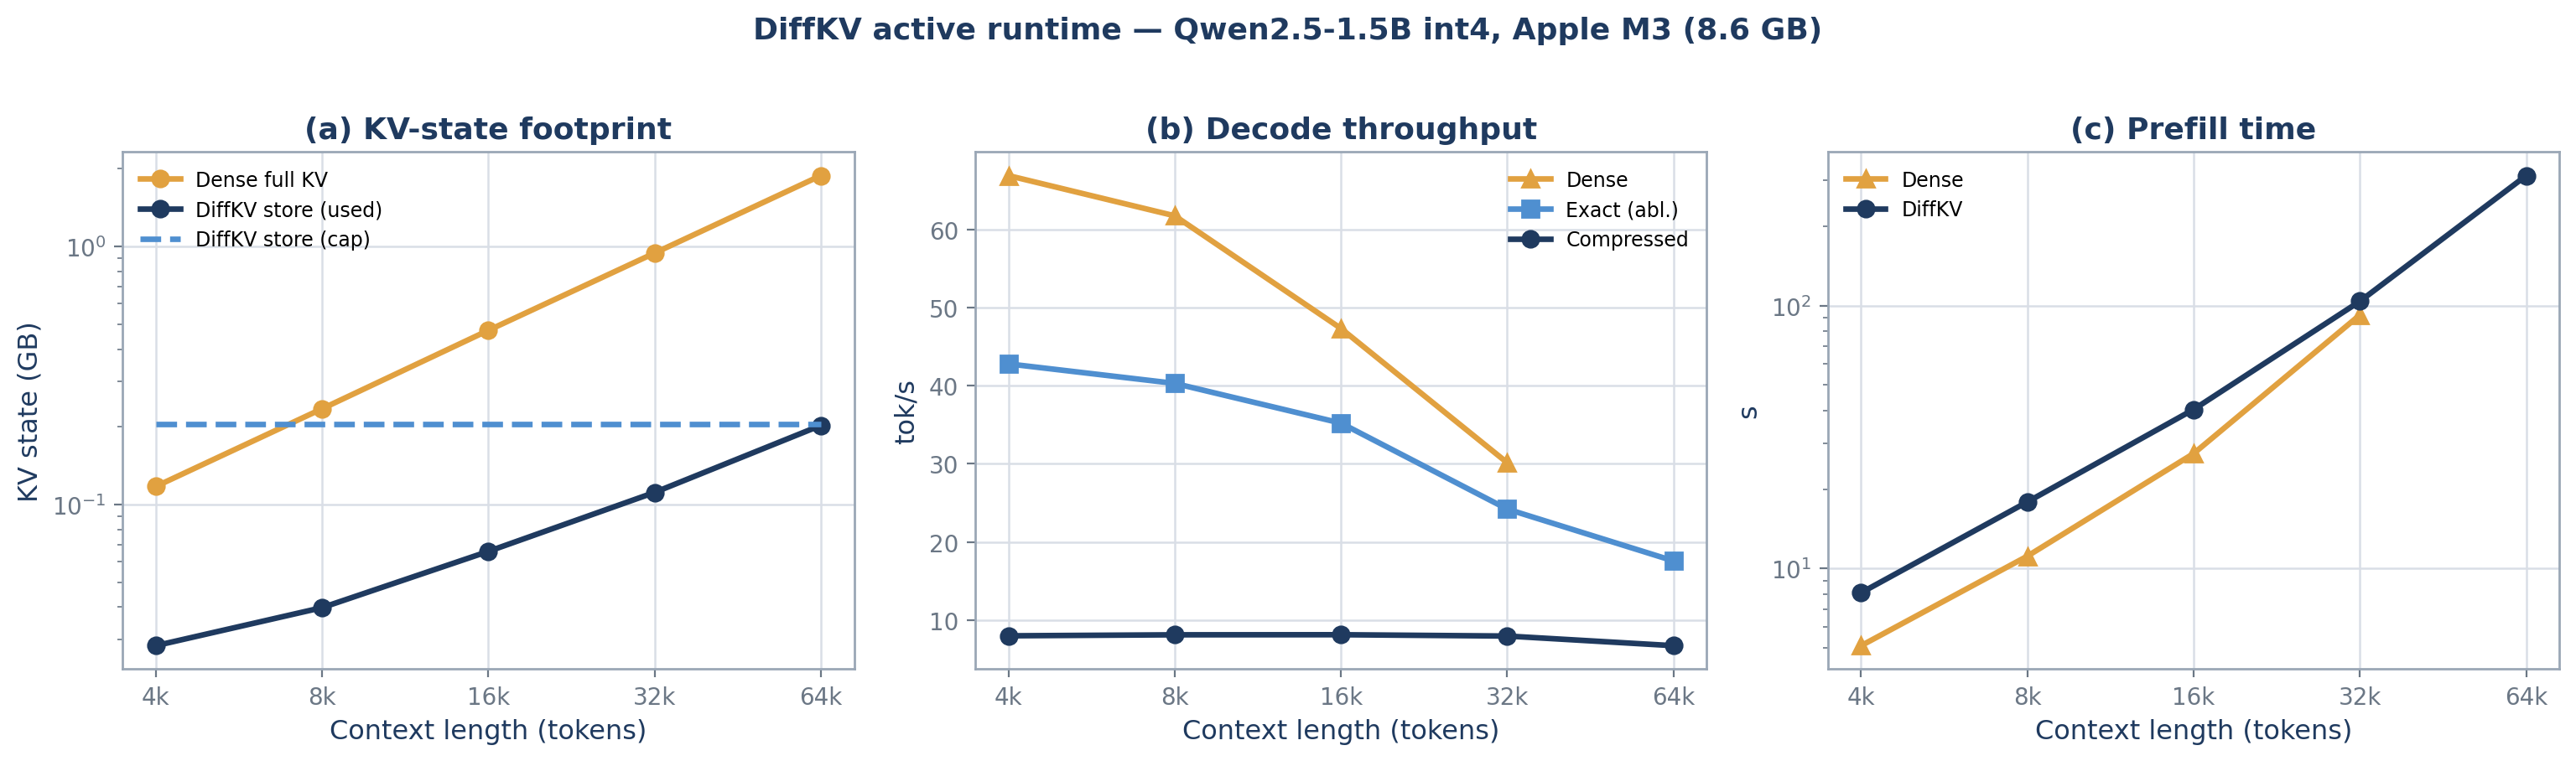
\includegraphics[width=0.96\linewidth]{figures/g5_combined.png}
  \caption{Combined view: (a) KV-state footprint, (b) decode throughput, (c) prefill time, for
  \diffkv{} compressed, the exact ablation, and the dense baseline.}
  \label{fig:g5}
\end{figure*}
